\documentclass[12pt]{article}

\usepackage[utf8]{inputenc}
\usepackage[russian]{babel}
\usepackage{amsmath}
\usepackage{setspace}

\usepackage{caption}
\usepackage{subcaption}
\usepackage{float}
\usepackage{graphicx}
\graphicspath{ {./images/} }

\usepackage{geometry}
 \geometry{
 a4paper,
 left=20mm,
 right=20mm,
 top=20mm,
 bot=20mm,
 }

\begin{document}

\begin{titlepage}
\begin{center}
    {\small НАЦИОНАЛЬНЫЙ ИССЛЕДОВАТЕЛЬСКИЙ УНИВЕРСИТЕТ ИТМО} \\
    {\small Факультет систем управления и робототехники} \\
    \vspace*{10\baselineskip}
    {\LARGEЭлектроника и схемотехника} \\
    \ \\
    \begin{spacing}{1.5}
    {\large Лабораторная работа №8 \\
    Цифро-аналоговые и аналогово-цифровые преобразователи} \\
    \end{spacing} \\
    \ \\
    Вариант 2 \\
    \vspace*{10\baselineskip}
    \hfill {Выполнили студенты:} \\
    \hfill {Кирбаба Д.Д. R3338} \\
    \hfill {Курчавый В.В. R3338} \\
    \ \\
    \hfill {Преподаватель:} \\
    \hfill {Николаев Н.А.} \\
    \mbox{}
    \vfill {г. Санкт-Петербург\\2023}
\end{center}
\end{titlepage}

\section*{Цель работы}
Моделирование и исследование работы ЦАП на основе резистивной матрицы $R-2R$ и АЦП прямого (параллельного) действия в LTspice.

\section*{Ход работы}
Вариант 2.\\
Исходные данные для схемы ЦАП: разрядность $4$, операционный усилитель $AD711$, $R = 5 \ kOhm$. \\
Исходные данные для схема АЦП: компаратор $LT1018$, $V_{ref} = 10 \ V$.

\subsubsection*{Исследование работы ЦАП}

\begin{figure}[H]
    \centering
    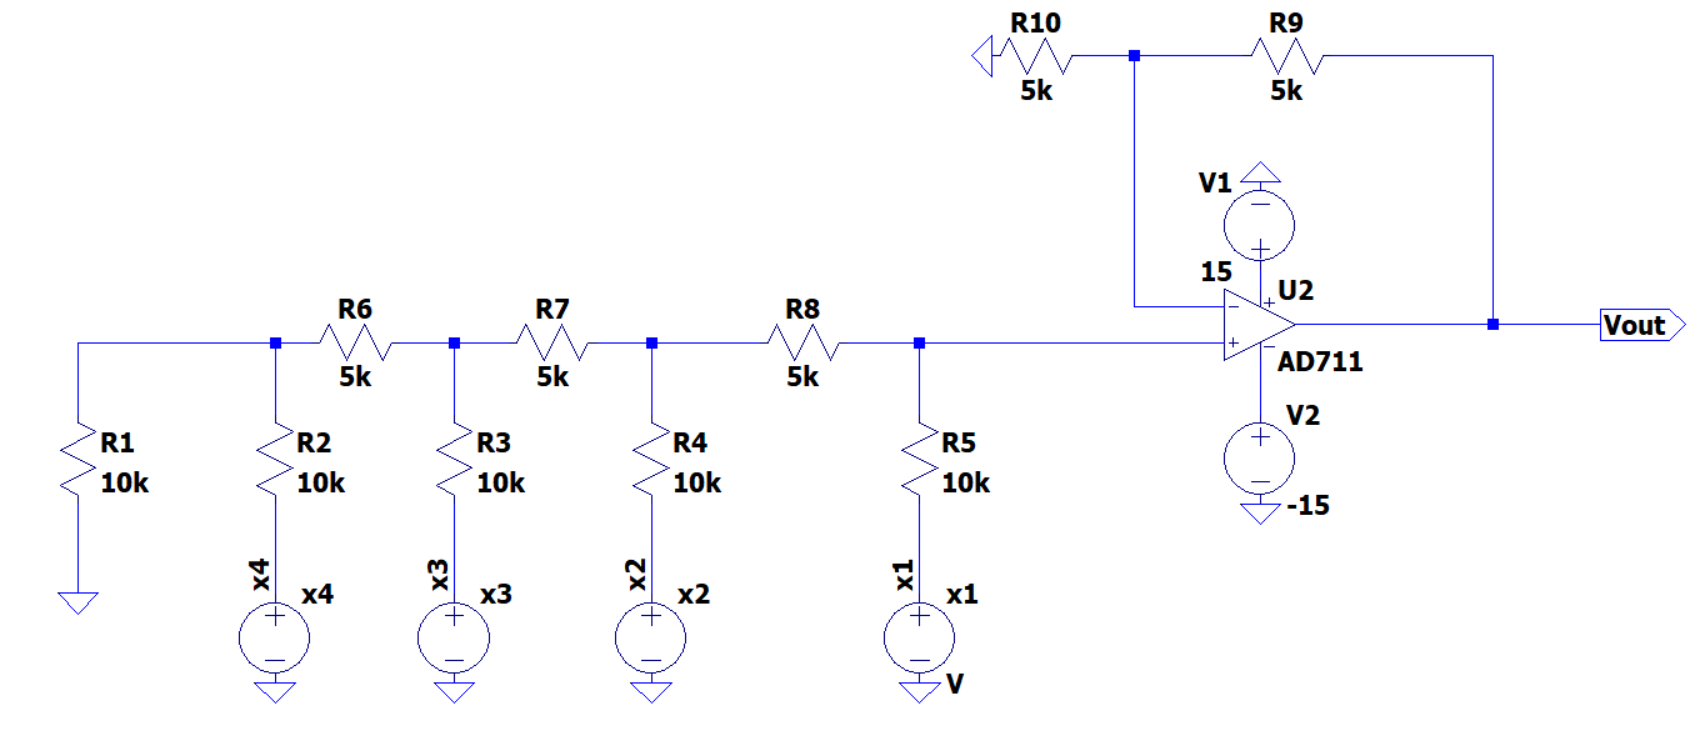
\includegraphics[width=\textwidth]{dac_scheme.png}
    \caption{Блок-схема ЦАП на основе резистивной матрицы $R-2R$.}
    \label{fig:dac_scheme}
\end{figure}

\begin{table}[H]
    \centering
    \begin{tabular}{c | c | c | c | c} 
        $x_4$ & $x_3$ & $x_2$ & $x_1$ & $V_{out}, \ V$ \\  
        \hline
        0 & 0 & 0 & 0 & $0$ \\ 
        \hline
        0 & 0 & 0 & 1 & $0.625$ \\ 
        \hline
        0 & 0 & 1 & 0 & $1.25$ \\ 
        \hline
        0 & 0 & 1 & 1 & $1.875$ \\ 
        \hline
        0 & 1 & 0 & 0 & $2.5$ \\ 
        \hline
        0 & 1 & 0 & 1 & $3.125$ \\ 
        \hline
        0 & 1 & 1 & 0 & $3.75$ \\ 
        \hline
        0 & 1 & 1 & 1 & $4.375$ \\ 
        \hline
        1 & 0 & 0 & 0 & $5$ \\ 
        \hline
        1 & 0 & 0 & 1 & $5.625$ \\ 
        \hline
        1 & 0 & 1 & 0 & $6.25$ \\ 
        \hline
        1 & 0 & 1 & 1 & $6.875$ \\ 
        \hline
        1 & 1 & 0 & 0 & $7.5$ \\ 
        \hline
        1 & 1 & 0 & 1 & $8.125$ \\ 
        \hline
        1 & 1 & 1 & 0 & $8.75$ \\ 
        \hline
        1 & 1 & 1 & 1 & $9.375$ \\ 
    \end{tabular}
    \caption{Таблица состояний ЦАП.}
    \label{table:1}
\end{table}

\begin{figure}[H]
    \centering
    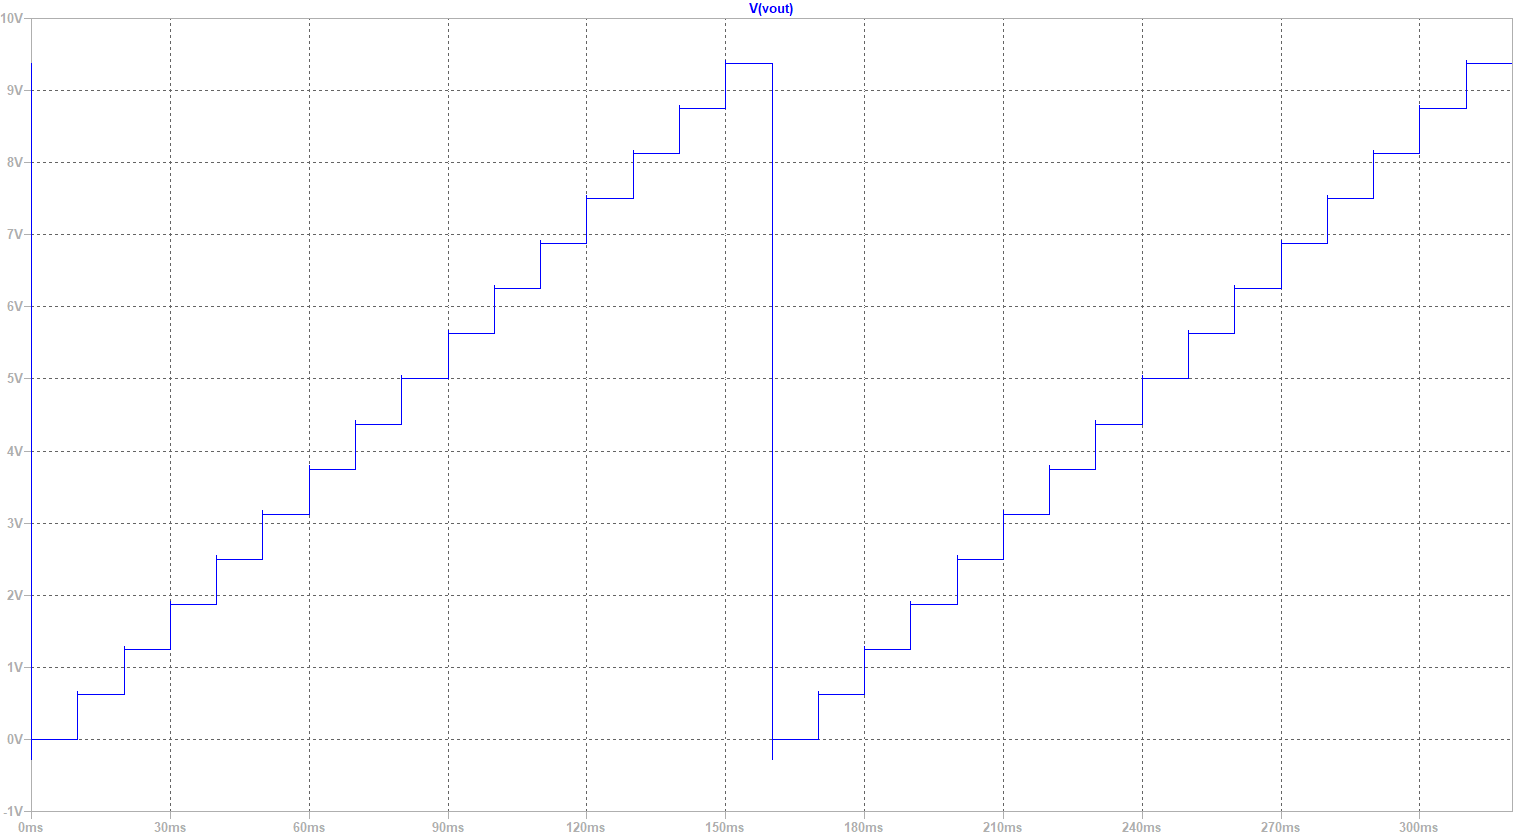
\includegraphics[width=\textwidth]{dac_out.png}
    \caption{График выходного сигнала.}
    \label{fig:dac_out}
\end{figure}

\begin{figure}[H]
    \centering
    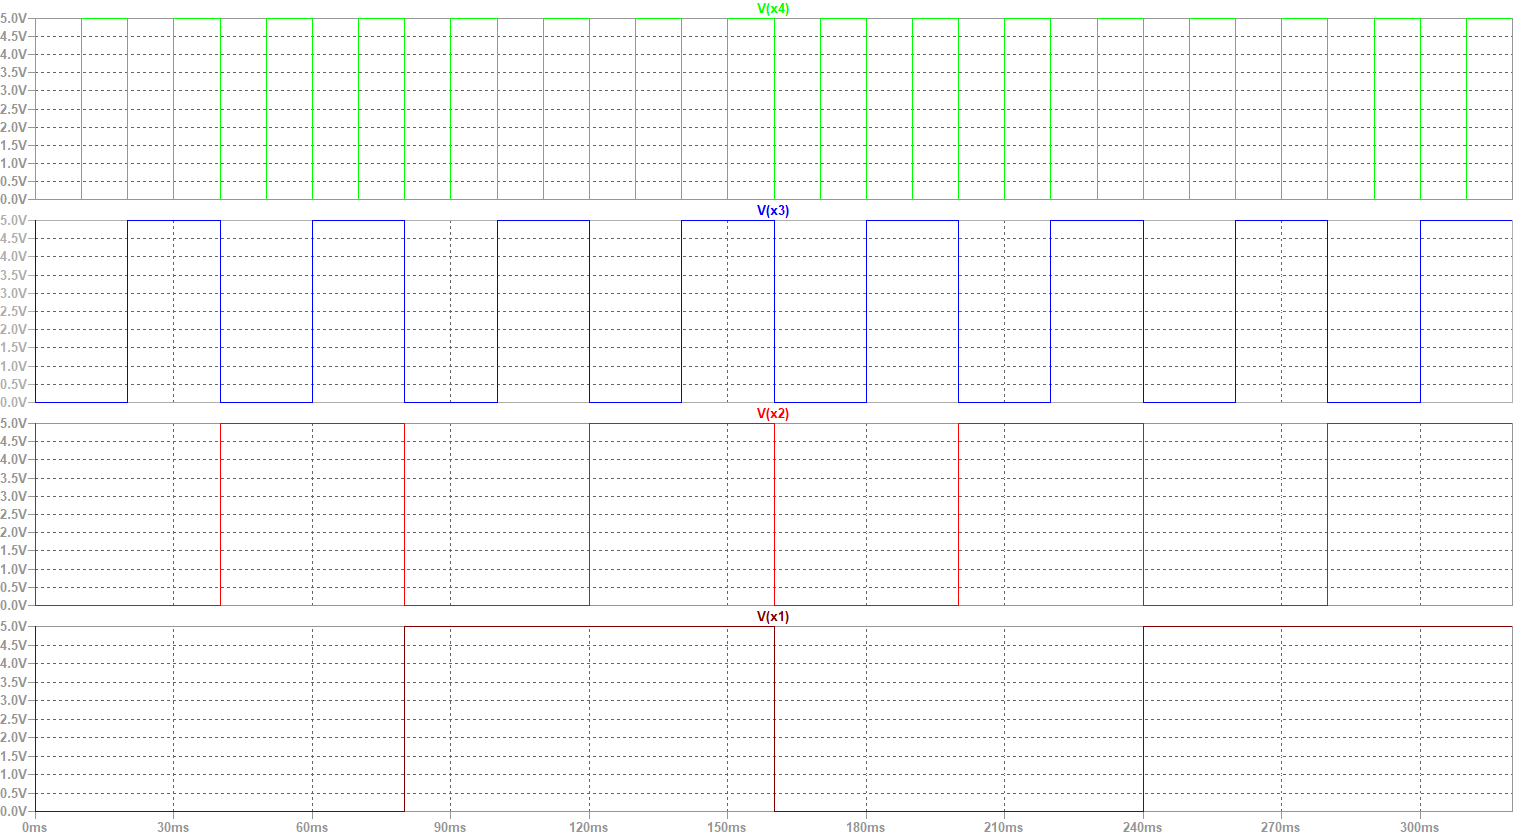
\includegraphics[width=\textwidth]{dac_bits.png}
    \caption{Графики входных сигналов.}
    \label{fig:dac_bits}
\end{figure}

\subsubsection*{Исследование работы АЦП}

\begin{figure}[H]
    \centering
    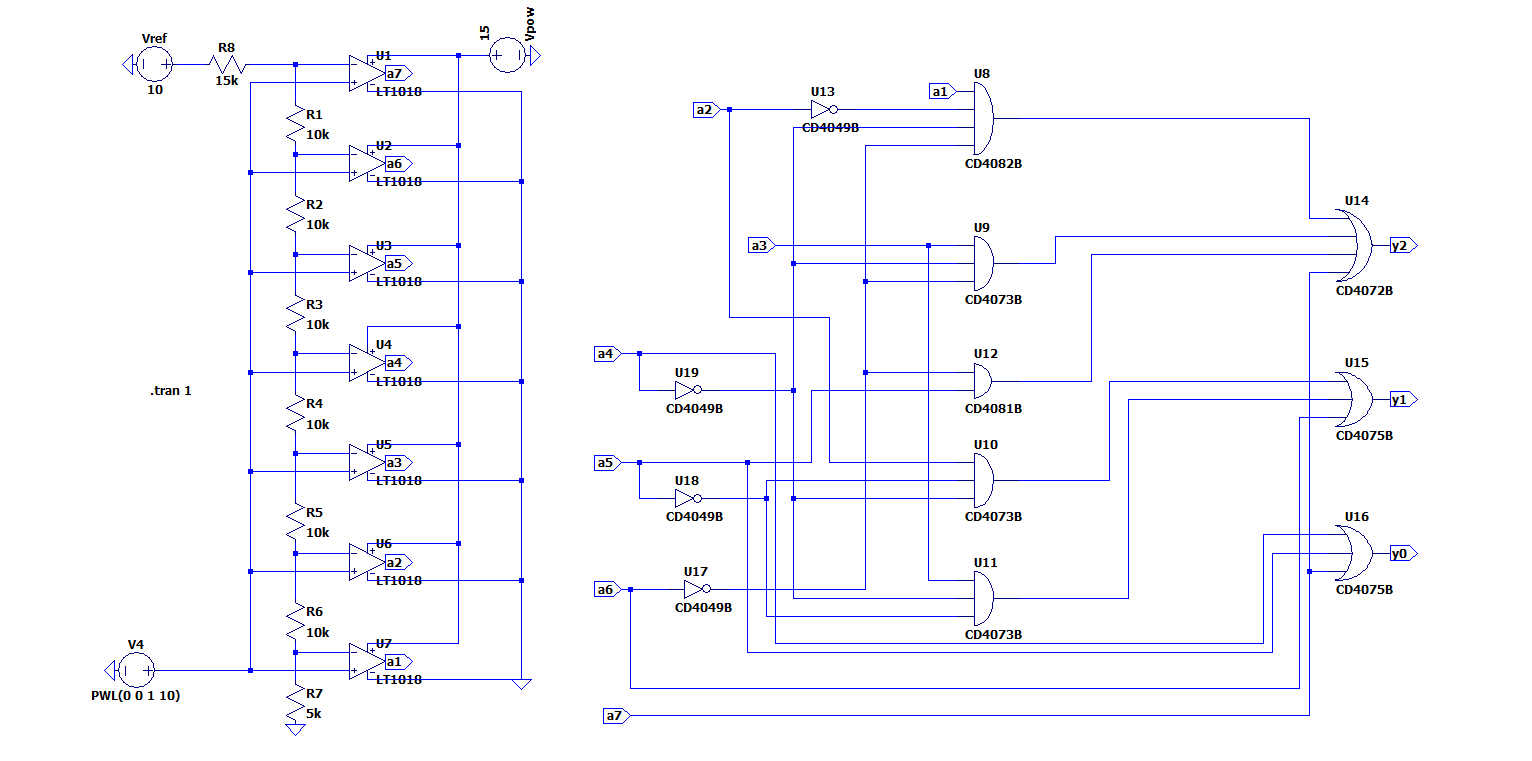
\includegraphics[width=\textwidth]{adc_scheme.png}
    \caption{Блок-схема прямого (параллельного) АЦП с приоритетным шифратором $8-3$.}
    \label{fig:adc_scheme}
\end{figure}

\begin{figure}[H]
    \centering
    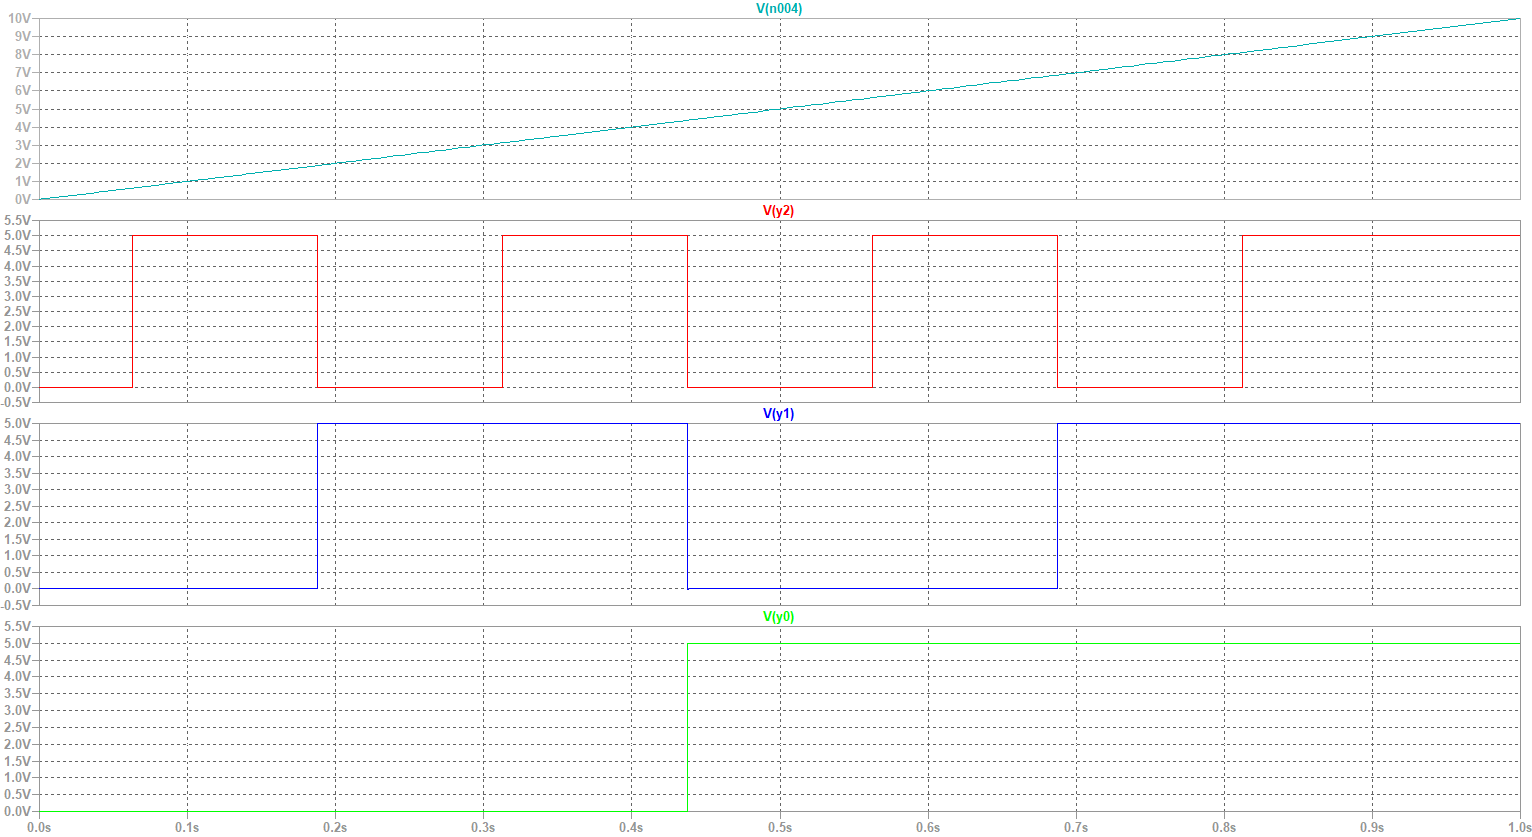
\includegraphics[width=\textwidth]{adc_in_out.png}
    \caption{Графики входных и выходных сигналов АЦП.}
    \label{fig:adc_in_out}
\end{figure}

\begin{table}[H]
    \centering
    \begin{tabular}{c | c | c | c} 
        $y_3$ & $y_2$ & $y_1$ & $V_{in}, \ V$ \\  
        \hline
        0 & 0 & 0 & $[V_{min}, \ 0.63]$ \\ 
        \hline
        0 & 0 & 1 & $(0.63, \ 1.875]$ \\ 
        \hline
        0 & 1 & 0 & $(1.875, \ 3.125]$ \\ 
        \hline
        0 & 1 & 1 & $(3.125, \ 4.375]$ \\ 
        \hline
        1 & 0 & 0 & $(4.375, \ 5.625]$ \\ 
        \hline
        1 & 0 & 1 & $(5.625, \ 6.877]$ \\ 
        \hline
        1 & 1 & 0 & $(6.877, \ 8.126]$ \\ 
        \hline
        1 & 1 & 1 & $(8.126, \ V_{max}]$ \\ 
    \end{tabular}
    \caption{Таблица состояний АЦП.}
    \label{table:1}
\end{table}

\section*{Выводы}
В данной работе исследовались ЦАП и АЦП. Это элементы выполняющие преобразование информации, содержащейся в аналоговом сигнале, в цифровой код и наоборот. \\
\ \\
В первой части работы была собрана схема ЦАП на основе резистивной матрицы $R-2R$ разрядности $4$, затем было произведено моделирование его работы в виде преобразования двоичных последовательностей в аналоговый сигнал. Результаты работы были оформлено в виде таблицы. Если соединить точки $V_{out}$, то получится статическая характеристика преобразователя, которая будет достаточно близка к идеальной (имеет вид прямой линии). \\
\ \\
Во второй части исследовался прямой АЦП с приоритетным шифратором $8-3$. Во время работы преобразователя выполняются следующие функции: временная дискретизация, квантование по уровню, кодирование. Принцип преобразования основан на последовательном сравнении уровня входного сигнала с уровнями сигналов соответствующих различным комбинациям выходного кода и формировании результирующего кода по результатам сравнений. \\
Была построена блок-схема АЦП, затем произведено моделирование при изменяющимся входном напряжении. В результате получены интервалы соответствующие определенным двоичным кодам, которые являются приближением непрерывного аналогово сингала подаваемого на вход.

\end{document}